\documentclass[tikz,border=6pt]{standalone}
% polymer-paper-preamble
\usepackage{fontspec}
\usepackage{amsmath}
\usetikzlibrary{arrows.meta,calc,decorations.pathmorphing,positioning,shapes.geometric}
\setmainfont{TeX Gyre Heros}
\setsansfont{TeX Gyre Heros}
\definecolor{cBlue}{HTML}{356CA5}
\definecolor{cRed}{HTML}{C94F45}
\definecolor{cTeal}{HTML}{258B82}
\definecolor{cAmber}{HTML}{D99A2B}
\definecolor{cBrown}{HTML}{7B5B46}
\definecolor{cGray}{HTML}{69737D}
\tikzset{
  font=\sffamily,
  panel/.style={draw=cGray!55,rounded corners=2pt,line width=.65pt},
  paneltitle/.style={font=\sffamily\bfseries\fontsize{9}{10}\selectfont,text=cGray!90!black},
  modulelabel/.style={font=\sffamily\bfseries\fontsize{7}{8}\selectfont,text=cGray!90!black},
  note/.style={font=\sffamily\fontsize{6.1}{7.1}\selectfont,text=cGray!95!black,align=center},
  tinylabel/.style={font=\sffamily\fontsize{5.4}{6.3}\selectfont,text=cGray!95!black,align=center},
  sulfur/.style={circle,draw=cAmber!85!black,fill=cAmber!22,minimum size=4.5mm,inner sep=0pt,line width=.7pt,font=\bfseries\scriptsize,text=cBrown},
  carbon/.style={circle,draw=cGray,fill=white,minimum size=3.7mm,inner sep=0pt,line width=.65pt,font=\scriptsize,text=cGray!90!black},
  bond/.style={draw=cBrown,line width=1.05pt},
  crosslink/.style={draw=cBlue,line width=1.25pt},
  energyaxis/.style={draw=cGray,line width=.8pt,-{Stealth[length=2.2mm]}},
  shallowtrap/.style={draw=cTeal,fill=cTeal!18,line width=.7pt},
  deeptrap/.style={draw=cRed,fill=cRed!16,line width=.75pt},
  evidencecurve/.style={draw=cBlue,line width=1.25pt},
  apparatus/.style={draw=cGray!90!black,line width=.85pt},
  sample/.style={draw=cBrown,fill=cBrown!13,line width=.8pt},
  electrode/.style={draw=cBlue!90!black,fill=cBlue!18,line width=.8pt},
  fieldarrow/.style={draw=cAmber!90!black,line width=.9pt,-{Stealth[length=2mm]}},
  forcearrow/.style={draw=cRed,line width=1.2pt,-{Stealth[length=2.4mm]}},
  circuit/.style={draw=cBlue!90!black,line width=.9pt},
  charge/.style={font=\bfseries\scriptsize,text=cRed}
}
\begin{document}
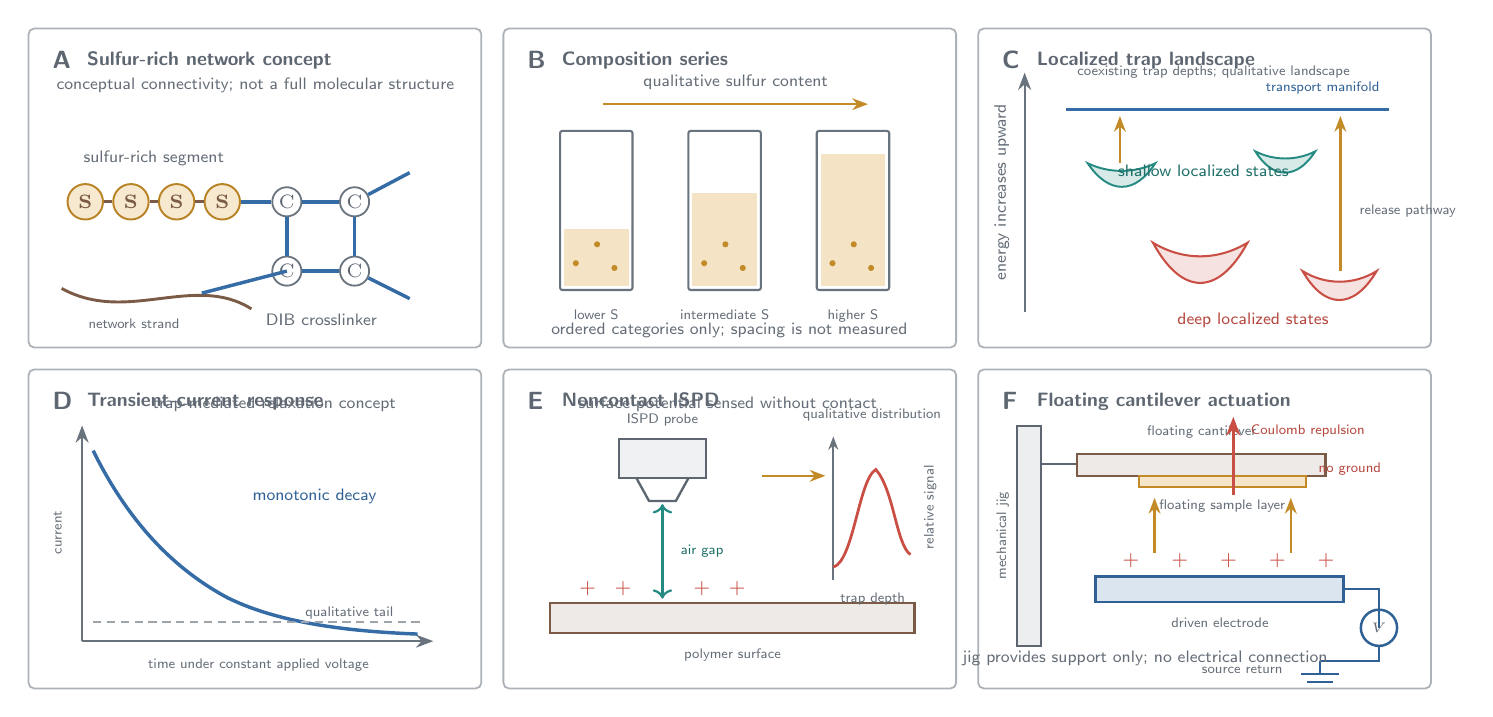
\begin{tikzpicture}[x=1cm,y=1cm]
  \def\PW{5.75}
  \def\PH{4.05}
  \def\GX{.28}
  \def\GY{.28}
  \foreach \x/\y/\letter/\title in {
    0/4.33/A/{Sulfur-rich network concept},
    6.03/4.33/B/{Composition series},
    12.06/4.33/C/{Localized trap landscape},
    0/0/D/{Transient-current response},
    6.03/0/E/{Noncontact ISPD},
    12.06/0/F/{Floating cantilever actuation}}
  {
    \draw[panel] (\x,\y) rectangle ++(\PW,\PH);
    \node[paneltitle,anchor=north west] at (\x+.18,\y+\PH-.16) {\letter};
    \node[modulelabel,anchor=north west] at (\x+.62,\y+\PH-.18) {\title};
  }

  % Panel A: semantic polymer repeat-unit concept
  \node[sulfur] (A-s1) at (.72,6.18) {S};
  \node[sulfur] (A-s2) at (1.30,6.18) {S};
  \node[sulfur] (A-s3) at (1.88,6.18) {S};
  \node[sulfur] (A-s4) at (2.46,6.18) {S};
  \draw[bond] (A-s1)--(A-s2)--(A-s3)--(A-s4);
  \node[note,anchor=south] at (1.59,6.52) {sulfur-rich segment};
  \node[carbon] (A-c1) at (3.28,6.18) {C};
  \node[carbon] (A-c2) at (4.14,6.18) {C};
  \node[carbon] (A-c3) at (4.14,5.30) {C};
  \node[carbon] (A-c4) at (3.28,5.30) {C};
  \draw[crosslink] (A-s4)--(A-c1)--(A-c2)--(A-c3)--(A-c4)--(A-c1);
  \draw[crosslink] (A-c2)--(4.84,6.55) (A-c3)--(4.84,4.95);
  \node[note,anchor=north] at (3.72,4.88) {DIB crosslinker};
  \draw[bond] (.42,5.08) .. controls (1.25,4.62) and (2.10,5.28) .. (2.83,4.82);
  \draw[crosslink] (2.20,5.02)--(3.28,5.30);
  \node[tinylabel] at (1.34,4.63) {network strand};
  \node[note] at (2.88,7.66) {conceptual connectivity; not a full molecular structure};

  % Panel B: qualitative sulfur-composition series
  \foreach \x/\h/\lab in {6.75/.72/{lower S},8.38/1.18/{intermediate S},10.01/1.68/{higher S}} {
    \draw[draw=cGray,line width=.75pt,rounded corners=.8pt] (\x,5.06) rectangle ++(.92,2.02);
    \fill[cAmber!28] (\x+.05,5.11) rectangle ++(.82,\h);
    \foreach \dx/\dy in {.20/.24,.47/.48,.69/.18} {
      \fill[cAmber!90!black] (\x+\dx,5.16+\dy) circle (1.1pt);
    }
    \node[tinylabel,anchor=north] at (\x+.46,4.93) {\lab};
  }
  \draw[fieldarrow] (7.30,7.42)--(10.66,7.42);
  \node[note,anchor=south] at (8.98,7.48) {qualitative sulfur content};
  \node[note] at (8.90,4.55) {ordered categories only; spacing is not measured};

  % fig-agent:start panel-c-trap-landscape
  % Panel C: hero trap landscape
  \draw[energyaxis] (12.65,4.78)--(12.65,7.82);
  \node[note,rotate=90] at (12.36,6.30) {energy increases upward};
  \draw[draw=cBlue,line width=1.25pt] (13.18,7.35)--(17.28,7.35);
  \node[tinylabel,anchor=south east,text=cBlue!90!black] at (17.28,7.42) {transport manifold};
  \path[shallowtrap] (13.45,6.67) .. controls (13.72,6.27) and (14.05,6.27) .. (14.31,6.67)
    .. controls (14.04,6.54) and (13.72,6.54) .. cycle;
  \path[shallowtrap] (15.58,6.82) .. controls (15.80,6.46) and (16.11,6.46) .. (16.34,6.82)
    .. controls (16.10,6.70) and (15.82,6.70) .. cycle;
  \path[deeptrap] (14.28,5.66) .. controls (14.65,4.98) and (15.11,4.98) .. (15.48,5.66)
    .. controls (15.10,5.43) and (14.66,5.43) .. cycle;
  \path[deeptrap] (16.18,5.30) .. controls (16.46,4.81) and (16.83,4.81) .. (17.12,5.30)
    .. controls (16.83,5.12) and (16.47,5.12) .. cycle;
  \node[note,text=cTeal!80!black] at (14.92,6.57) {shallow localized states};
  \node[note,text=cRed!90!black] at (15.55,4.67) {deep localized states};
  \draw[fieldarrow] (13.86,6.67)--(13.86,7.27);
  \draw[fieldarrow] (16.66,5.30)--(16.66,7.27);
  \node[tinylabel,anchor=west] at (16.78,6.06) {release pathway};
  \node[tinylabel] at (15.05,7.83) {coexisting trap depths; qualitative landscape};
  % fig-agent:end panel-c-trap-landscape

  % Panel D: qualitative transient current
  \draw[energyaxis] (.68,.60)--(.68,3.34);
  \draw[energyaxis] (.68,.60)--(5.14,.60);
  \node[tinylabel,rotate=90] at (.37,1.98) {current};
  \node[tinylabel] at (2.92,.30) {time under constant applied voltage};
  \draw[evidencecurve] (.82,3.02) .. controls (1.20,2.25) and (1.74,1.57) .. (2.53,1.15)
    .. controls (3.24,.80) and (4.20,.72) .. (4.94,.69);
  \draw[densely dashed,draw=cGray!65,line width=.6pt] (.82,.84)--(4.98,.84);
  \node[note,anchor=west,text=cBlue!90!black] at (2.72,2.44) {monotonic decay};
  \node[tinylabel,anchor=west] at (3.39,.96) {qualitative tail};
  \node[note] at (3.12,3.61) {trap-mediated relaxation concept};

  % Panel E: noncontact ISPD and interpretation
  \draw[sample] (6.62,.70) rectangle (11.25,1.08);
  \node[tinylabel,anchor=north] at (8.94,.62) {polymer surface};
  \node[apparatus,fill=cGray!10,minimum width=1.10cm,minimum height=.50cm] (E-probe) at (8.05,2.92) {};
  \draw[apparatus] (7.72,2.67)--(7.88,2.38)--(8.22,2.38)--(8.38,2.67);
  \node[tinylabel,anchor=south] at (8.05,3.21) {ISPD probe};
  \draw[<->,draw=cTeal,line width=.8pt] (8.05,1.14)--(8.05,2.34);
  \node[tinylabel,anchor=west,text=cTeal!80!black] at (8.16,1.74) {air gap};
  \foreach \x in {7.10,7.55,8.55,9.00} {\node[charge] at (\x,1.27) {$+$};}
  \draw[fieldarrow] (9.32,2.70)--(10.12,2.70);
  \draw[draw=cGray,line width=.65pt,-{Stealth[length=1.7mm]}] (10.22,1.38)--(10.22,3.20);
  \path[draw=cRed,line width=1pt] (10.22,1.54) .. controls (10.48,1.62) and (10.54,2.65) .. (10.76,2.78)
    .. controls (10.99,2.52) and (11.02,1.82) .. (11.20,1.70);
  \node[tinylabel,anchor=north] at (10.72,1.34) {trap depth};
  \node[tinylabel,rotate=90] at (11.45,2.30) {relative signal};
  \node[note] at (8.88,3.61) {surface potential sensed without contact};
  \node[tinylabel] at (10.71,3.47) {qualitative distribution};

  % fig-agent:start panel-f-electrical-topology
  % Panel F: mechanical jig, floating cantilever, driven lower electrode
  \draw[apparatus,fill=cGray!12] (12.55,.54) rectangle (12.86,3.33);
  \node[tinylabel,rotate=90] at (12.37,1.94) {mechanical jig};
  \draw[apparatus] (12.86,2.85)--(13.31,2.85);
  \draw[sample] (13.31,2.70) rectangle (16.47,2.98);
  \fill[cAmber!25,draw=cAmber!90!black,line width=.65pt] (14.10,2.56) rectangle (16.22,2.70);
  \node[tinylabel,anchor=south] at (14.90,3.05) {floating cantilever};
  \node[tinylabel,anchor=north] at (15.16,2.52) {floating sample layer};
  \node[tinylabel,text=cRed!90!black] at (16.78,2.78) {no ground};
  \draw[forcearrow] (15.30,2.46)--(15.30,3.45);
  \node[tinylabel,anchor=west,text=cRed!90!black] at (15.40,3.27) {Coulomb repulsion};
  \draw[electrode] (13.55,1.10) rectangle (16.70,1.42);
  \node[tinylabel,anchor=north] at (15.13,1.02) {driven electrode};
  \foreach \x in {14.00,14.62,15.24,15.86,16.48} {\node[charge] at (\x,1.62) {$+$};}
  \draw[fieldarrow] (14.30,1.72)--(14.30,2.42);
  \draw[fieldarrow] (16.03,1.72)--(16.03,2.42);
  \draw[circuit] (16.70,1.26)--(17.15,1.26)--(17.15,.77);
  \draw[circuit] (17.15,.77) circle (.23);
  \node[tinylabel] at (17.15,.77) {$V$};
  \draw[circuit] (17.15,.54)--(17.15,.35)--(16.40,.35);
  \draw[circuit] (16.40,.35)--(16.40,.18);
  \draw[circuit] (16.16,.18)--(16.64,.18);
  \draw[circuit] (16.23,.08)--(16.57,.08);
  \node[tinylabel,anchor=east] at (16.05,.24) {source return};
  \node[note] at (14.18,.38) {jig provides support only; no electrical connection};
  % fig-agent:end panel-f-electrical-topology
\end{tikzpicture}
\end{document}
